\documentclass[12pt]{memoir}
\usepackage{amsfonts}
\usepackage{amsmath}
\usepackage{tikz}
\usepackage{multicol}
\usetikzlibrary{trees,positioning,fit,arrows,decorations.pathreplacing}
\usepackage[paperwidth=12in]{geometry}
\begin{document}
In our context, Firstly the Rainbow DQN can only distinguish between states which have different board states, and thus doesn’ know about time, second we construct the environmental  health graphs to be. Because the island navigation environment we are investigating only has two states, we labelled them life and death for convenience. \\
\begin{center}
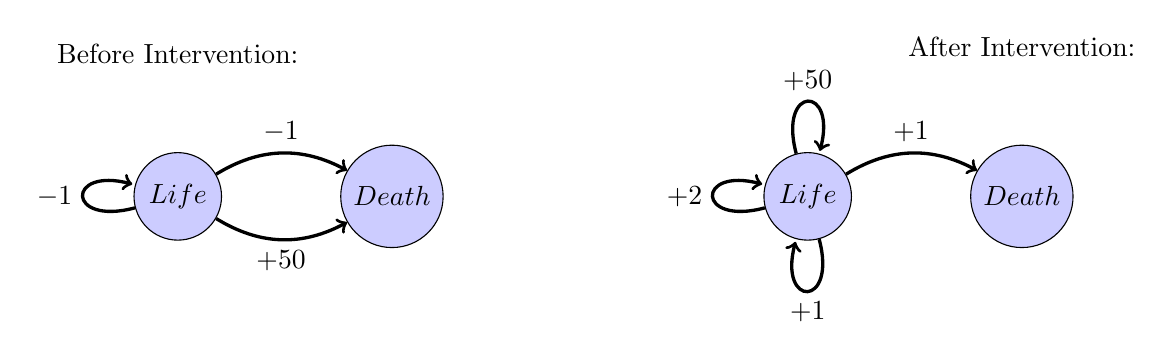
\begin{tikzpicture}
    \tikzset{main node/.style = {circle, fill =blue!20, draw}}
    \node[main node] (l) {$Life$};
    \node[main node] (d) [ right =  1.5cm of l]  {$Death$};
    \node (title) [right = 0.75cm of l, above = 1cm of l] {Before Intervention:};
    \path[->, very thick] 
   %FROM Bend/Loop   position of label   label    to
    (l) edge[bend left] node[midway, above] {$-1$} (d)
    (l) edge[bend right] node[midway, below] {$+50$}(d)
    (l) edge[loop left] node[midway, left] {$-1$} (l)
   ;
    %%
    \begin{scope}[xshift=8cm]
     \node[main node] (L) {$Life$};
    \node[main node] (D) [right =  1.5cm of L]  {$Death$}; \node (title) [above = 1cm of D] {After Intervention:};
    \path[->, very thick] 
    (L) edge[bend left] node[midway, above] {$+1$} (D) 
    (L) edge[loop above] node[midway, above] {$+50$} (L)
    (L) edge[loop below] node[midway,below] {$+1$} (L)
    (L) edge[loop left] node[midway,left] {$+2$} (L);
    \end{scope}
\end{tikzpicture}
\end{center}

 Now we apply the intervention, by giving the agent 2 additional points every second it is alive, and by having the goal being hit changed to the goal being discovered in that episode. 
 \begin{multicols}{2}
 	Before Intervention: \\
 $$ R_a(s,s') =  \begin{cases}
 +50 & if \:  s' \textrm{ is the goal } \\ 
 -1    &  \textrm{ always while alive }
 \end{cases} $$
  \columnbreak
   \\
   After Intervention: \\
   $$\quad R_a(s,s') = \begin{cases}
   +50 & if \: s' \textrm{ is the goal (only the first time in the episode) } \\ 
   -1    & if \: s' \textrm{ is not goal } \\  
   +2   & \textrm{ always while alive }
    \end{cases} $$
\end{multicols}


\end{document}